\section{User model} 
\label{sec:user_model}

We consider many users owning several devices, that they freely turn on and off depending on their location and will.
The participants' devices are the only nodes constituting our system; the unreliability of their connectivity has to be taken for granted.

We will first present a model of each user's behavior, that will drive the connection intervals of our system's nodes.

\subsection{A model of the user's behavior}
\label{sub:a_model_of_the_user_s_behavior}

In \name, we take interest in users that own several devices, and wish to privately exchange files with each other.
To the best of our knowledge, no real-world traces of multi-devices usage over several days exist, as would be needed for the experimental evaluation of our system.
For that reason, we propose a user behavioral model having the following features:

\begin{itemize}
	\item Each user owns a variable amount of devices, that can be either mobile or immobile;
	\item The user travels between three ``locations'' according to a simple probabilistic model: her home, her workplace, and outside;
	\item She can act on her devices only when she is close to them. For instance, a user cannot shut down her workstation while being home or outside.
\end{itemize}

To this end, we use a Hidden Markov Model (HMM). 
The \emph{hidden} Markovian process $S=S_1,\dots,S_T$ represents the user's progression among the three proposed locations.
The \emph{observable} process $O=O_1,\dots,O_T$ reads ``toggle'' actions performed by the user on her devices. The probability of observable events depends on the current location.
For instance, the probability that the user switches her home computer on or off is null while she is at work or outside.

Such a statistical model is simplistic (e.g. it does not encapsulate date \& time nor location), but it is on purpose: simplicity is bliss.
Given the lack of real-world data for our testbed, building a more complex and realistic user model would add no value to our proposal: 
our goal is to see devices exhibiting frequent disconnections and reconnections (also called \emph{churn}).
Our simple model being able to put extravagant stress on our system, it is sufficient to access \name's resilience.

\subsubsection{Formal definition} % (fold)
\label{ssub:formal_definition}


\begin{figure}[t]
\centering
\vspace{-1em}

$$A =
\kbordermatrix{
      & W            & O            & H            \cr
    W & \sfrac{2}{3} & \sfrac{1}{3} & 0            \cr
    O & \sfrac{1}{3} & \sfrac{1}{3} & \sfrac{1}{3} \cr
    H & 0            & \sfrac{1}{3} & \sfrac{2}{3} \\[0.3em]
}, \;
B = 
\kbordermatrix{
      & W    & O    & H    \cr
    t_n & 0.1  & 0.45 & 0.1  \cr
    t_p & 0.45 & 0.55 & 0.45 \cr
    t_w & 0.45 & 0    & 0    \cr
    t_h & 0    & 0    & 0.45 \\[0.3em]
}$$

\includegraphics[width=0.9\columnwidth]{figures/hmm.pdf}
\caption{ \label{fig:hmm} Example Hidden Markov Model (HMM) of a user's behavior.}
\end{figure}

We consider a single user, owning a set of $\mathcal{D}$ devices.
Time is discretized here, and the user's activity is sequential: she can do zero or one action per ``round''of $T$s.
A HMM $\lambda_N$, comprising a set of states $\mathcal{S}$ and a set of observable events $\mathcal{O}$, is defined as follows:

$$\text{HMM}:\;\lambda_N=(\Pi, A, B)$$

where 
\begin{itemize}
	\item $N$ is the number of states in the system:
	$N = \left| \mathcal{S} \right|$;

	\item $\Pi=\left\{ \pi_i\right\}_{i\in\mathcal{S}}$ is the initial state distribution:\\
	$\pi_i=P[S_1=i]$;

	\item $A = \left\{ a_{ij}\right\}_{(i,j)\in\mathcal{S}^2}$ is the transition probability matrix:\\
	$a_{ij}=P[S_t=j \mid S_{t-1}=i]$;

	\item $B = \left\{ b_{ik}\right\}_{(i,k)\in\mathcal{S}\times\mathcal{O}}$ is the matrix of states conditional densities:
	$b_{ik} = P[O_t=k \mid S_t = i]$.
\end{itemize}

In our case, the states are the different locations where the user is susceptible to go.
We considered the three following locations: $\mathcal{S}=\left\{ \mathit{work}, \mathit{outside}, \mathit{home} \right\}$. 
There is one action per device $d\in\mathcal{D}$, plus a ``none'' action when the user does not do anything: 
$\mathcal{O} = \left\{ t_d \right\}_{d\in \mathcal{D}} \bigcup \left\{ t_\text{none} \right\}$.
$t_d$ means that the user turned her device $d$ on or off (i.e. \emph{toggled} it), depending on the device's previous state.

In figure~\ref{fig:hmm}, we show an example HMM of a user's behavioral HMM, along with its graphical representation (the initial state distribution $\Pi$ was left out for simplicity). 
The represented user possesses a phone, that she carries around with her, a home computer, that is only accessible from her home, and a workstation, located at her workplace.

\begin{figure}[t]
\centering
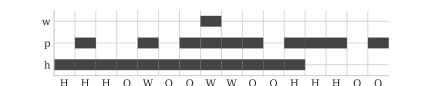
\includegraphics[width=\columnwidth]{figures/sample_usage.pdf}

\caption{\label{fig:sample_usage}Sample device usage using the previous HMM specifications. 
%The bottom line reads the HMM's states: \textbf{W}ork, \textbf{O}utside, and \textbf{H}ome, while the dark lines read when the devices (\textbf{h}ome computer, \textbf{p}hone, and \textbf{w}orkstation) are online.
}

\end{figure}

Using the toggle events, we compute the device's \emph{connection} events, represented by the multivariate Bernoulli process $C=\left\{ c^{(d)} \right\}_{d\in\mathcal{D}}$. 
$c^{(d)}_t=1$ (resp. 0) means that the device $d$ was online (resp. offline) at time step $t$.

We state that every device starts offline, and compute $c^{(d)}_t$ as follows:

$$ \forall d \in \mathcal{D},
\begin{cases}
c^{(d)}_t=0 &\text{when } t=0; \\
c^{(d)}_t=c^{(d)}_{t-1} \oplus \left[ O_t = t_d \right] &\text{when } t>0.
\end{cases}$$

Figure~\ref{fig:sample_usage}, shows a possible trace of the user's behavior, using the parameters depicted in figure~\ref{fig:hmm}. It read the timeline of $c^{(d)}$ for each device $d$. On the bottom of the graph, the first letter of the user's location is shown at each time step. We see that any number of devices can be connected at the same time.

% Each device starts offline; then, the user either toggles one device per round or does nothing.
% In this figure, we show the device \emph{usage}, that is a consequence of the $\mathit{toggle}$ events defined by the HMM.
% As a consequence, several devices can be online at the same time, as happens in the figure.



% subsubsection formal_definition (end)